\chapter{Trabalhos Relacionados}

\section{Vemcar}

%Desenvolvido na Universidade Federal do Rio Grande do Norte, o aplicativo Vemcar começou a ser desenvolvido em uma disciplina oferecida no curso de Engenharia de Software, logo após, o protótipo passou para a equipe da Superintendência de Informática da Universidade Federal do Rio Grande do Norte (SINFO), lá foi realizado toda a validação da ideia, surgimento dos requisitos e foram aplicadas as regras do um processo de software. No Vemcar somentes pessoas ligadas à universidade( professores, alunos, técnicos) podem utilizar o aplicativo.
O aplicativo Vemcar foi desenvolvido no Universidade Federal do Rio Grande do Norte. Foi desenvolvido inicialmente como parte do curso de Engenharia de Software, antes de o protótipo ser entregue à equipe da Superintendência de Ciência da Computação do Universidade Federal do Rio Grande do Norte (SINFO), onde ocorreu toda a validação da ideia, a criação dos requisitos e a aplicação das regras de um processo de software. Na Vemcar, somente pessoas relacionadas a universidade (professores, alunos, técnicos) podem utilizar o aplicativo.

%texto escrito por mim

\begin{figure}[!hbtp]
	\centering
	\caption{Aplicativo de Carona Solidária Vemcar}
	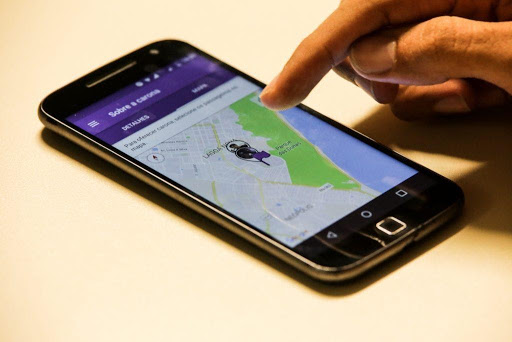
\includegraphics[width=0.6\textwidth]{./04-figuras/vemcar.jpg}
	\label{fig:tecnologia}
	\fonte{https://www.ufrn.br/imprensa/materias-especiais/2872/aplicativo-de-caronas-solidarias-da-ufrn-registra-mil-downloads-em-uma-semana}
\end{figure}

\section{RideUFF}

\section{Caronaphone}


\section{Caronaê}

%mencionar trabalho da luísa e do artigo publicado sobre o aplcativo.

%O Caronaê é um aplicativo de carona voltada para o ambiente universitário desenvolvido por alunos da Universidade Federal do Rio de Janeiro (UFRJ). O aplicativo está disponível para duas plataformas, Android e iOS. Em seu site oficial (CARONAÊ, 2020) diz que \textit{“O Caronaê é um sistema de código aberto, seguro e prático de caronas compartilhadas, criado com o objetivo de ser replicado em diferentes instituições e feito exclusivamente para a comunidade acadêmica das instituições integrantes da Rede Caronaê”}.
O Caronaê é um aplicativo de carona desenvolvido por alunos da Faculdade Federal do Rio de Janeiro (UFRJ) e voltado para o ambiente universitário. O aplicativo está disponível para duas plataformas, Android e iOS. O site oficial afirma que Caronaê é um sistema de carona aberto, seguro e prático, desenvolvido com o objetivo de ser replicado em diferentes instituições e exclusivamente para a comunidade acadêmica das instituições que pertencem à rede Caronaê (CARONAÊ, 2020).

%Dos pontos interessantes que o aplicativo oferece são, o uso exclusivo da comunidade acadêmica, a centralização das ofertas de carona, o aumento da taxa de ocupação dos veículos e pontos de carona para facilitar o encontro de caroneiro e carona. A Figura~\ref{fig:caronae} mostra a tela inicial do site do aplicativo de carona \textbf{Caronaê}.
Os pontos de interesse oferecidos pelo aplicativo incluem uso exclusivo pela comunidade acadêmica, centralização da oferta de caronas, aumento da utilização de veículos e pontos de carona para facilitar o encontro de caronas e caroneiros. Na Figura ~\ref{fig:caronae} temos a propaganda do aplicativo no site oficial. %podemos ver a tela inicial do aplicativo.mostra a tela inicial do site do aplicativo Caronaê.

\begin{figure}[!hbtp]
	\centering
	\caption{Aplicativo de Carona Solidária Caronaê}
	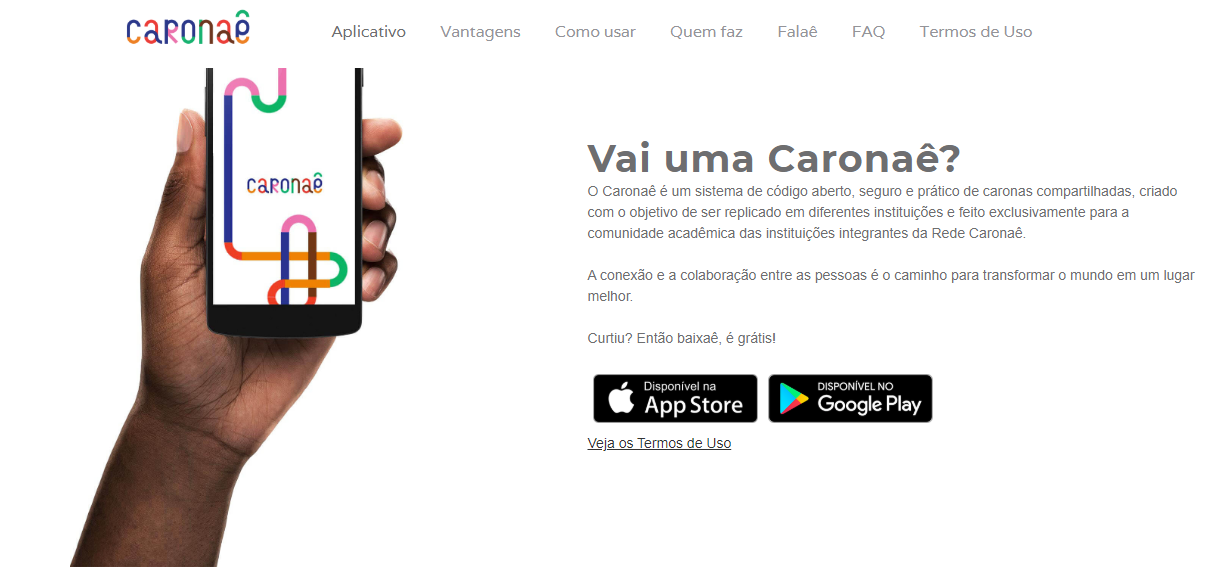
\includegraphics[width=0.8\textwidth]{./04-figuras/caronae.png}
	\label{fig:caronae}
	\fonte{https://caronae.org/index.html}
\end{figure}

\section{Waze Carpool}
Aplicativo das Empresas Waze, o \textit{Waze Carpool} é uma variante dos serviços da Waze que oferece compartilhamento de caronas entre seus usuários. O serviço oferecido pela empresa funciona através de um programa de parcerias. O aplicativo é bem dinâmico e intuitivo. A empresa aproveita os dados do aplicativo Waze para alimentar a dinâmica de navegação do Waze Carpool. como mostra a tela de grupos do aplicativo na Figura~\ref{fig:tela_grupos_wazecarpool}.

\begin{figure}[!hbtp]
	\centering
	\caption{Tela de grupos do aplicativo Waze Carpool}
	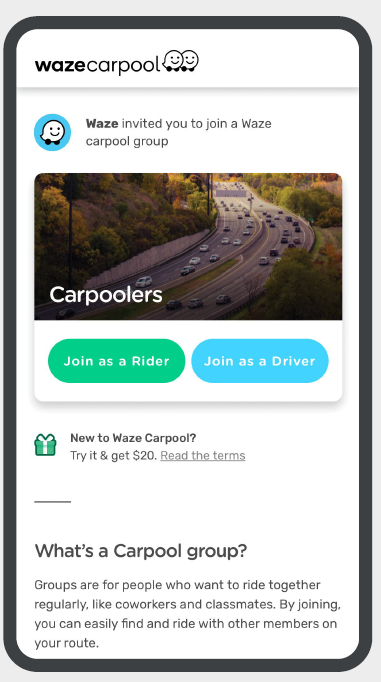
\includegraphics[width=0.3\textwidth]{./04-figuras/waze/Tela_de_grupos.png}
	\label{fig:tela_grupos_wazecarpool}
	\fonte{Programa de Parceria Brasil - Waze Carpool}
\end{figure}

%A Waze oferece o serviço do aplicativo para diversas empresas que desejam incorporar a cultura das caronas entre seus empregados porque a empresa acredita que as caronas costumam aproximar mais as pessoas e criar momentos que no local de trabalho não existiriam.
O Waze oferece um aplicativo para várias empresas que incorporam uma cultura de carona entre seus funcionários, pois a empresa acredita que a carona aproxima as pessoas e cria momentos que não existem no local de trabalho.

%O aplicativo tem uma dinâmica interessante, funciona a partir da criação de grupos, e os usuários destes grupos oferecem caronas entre si. Alunos de universidades como a UFRJ que por um tempo teve o seu próprio aplicativo de carona, o Caronaê, utilizam a ferramenta para pegar e oferecer a carona aos integrantes dos grupos que são criados e gerenciados por uma pessoa que ficar responsável pela comunicação da instituição com a empresa, o chamado "Embaixador".
O aplicativo tem uma dinâmica interessante, pois funciona criando grupos, e os usuários desses grupos oferecem caronas uns aos outros. %Estudantes de universidades como a UFRJ, que há algum tempo tinha um serviço próprio de carona, usam a ferramenta para pegar membros de grupos e oferecer carona. 
Esses grupos são criados e administrados por um responsável pela comunicação da instituição com a empresa, chamado de "embaixador".
% texto do material da waze 


\section{Quadro Comparativo}


\begin{table}[]
	\centering
	\caption{Trabalhos Relacionados}
	\label{tab:quadro-comparativo}

	\resizebox{1.0\textwidth}{!}{
	\begin{tabular}{|l|l|l|l|l|l|l|}
		\hline
		& Caronaê Unifap & Vemcar & RideUFF & Caronaphone & Waze Carpool & Blablacar \\ \hline
		Oferecer/Solicitar
		Caronas &                &        &         &             &              &           \\ \hline
		Identificação dos 
		usuários &                &        &         &             &              &           \\ \hline
		Restrição do público       &                &        &         &             &              &           \\ \hline
		Custo da viagem            &                &        &         &             &              &           \\ \hline
		Plataforma                 &                &        &         &             &              &           \\ \hline
		Chat entre 
		usuários        &                &        &         &             &              &           \\ \hline
	\end{tabular}}
\end{table}